
% \documentclass[10pt]{article}
\documentclass[10pt,twocolumn]{article}
\setlength\columnsep{6mm}

\usepackage[english]{babel}
\usepackage[stretch=10, shrink=10]{microtype}
% \usepackage[a4paper]{geometry}
\usepackage[a4paper, total={6.5in, 9in}]{geometry}
\usepackage{caption}
\usepackage{subcaption}
\usepackage{amsmath}
\usepackage{multirow}
\usepackage{xcolor}
\usepackage{hyperref}
\usepackage{float}
\usepackage[linesnumbered,lined,commentsnumbered]{algorithm2e}
\usepackage{enumitem}
\usepackage{dblfloatfix}
\ifdefined\noimage  % For omitting images during build from CLI
    \usepackage[demo]{graphicx}
\else
    \usepackage{graphicx}
\fi

% Tighter vspace in enumerate/itemize
% \setlist{noitemsep,topsep=0pt,parsep=0pt,partopsep=0pt}

\hypersetup{  % Prevents colored boxes around \cite and \ref
    allbordercolors = {white}
}

\newcommand{\note}[2]{#1${}_{#2}$}
\newcommand{\notesharp}[2]{#1${}_{#2}^{\sharp}$}
\newcommand{\noteflat}[2]{#1${}_{#2}^{\flat}$}

\newcommand{\floor}[1]{\left \lfloor #1 \right \rfloor}
\newcommand{\ceil}[1]{\left \lceil #1 \right \rceil}
\newcommand{\round}[1]{\left \lfloor #1 \right \rceil}


\title{\textbf{Real-time monophonic guitar pitch estimation\\using 12 tuned concurrent Fourier transforms}}
\author{Luc de Jonckheere}
% \date{}

\begin{document}
\selectlanguage{english}

\maketitle


\section*{Abstract}
\textcolor{gray}{Short summary.}
\textcolor{red}{Note that even though we focus on guitar pitch estimation, the methods described in this thesis are general to all instruments and even singing. The only guitar specific thing is the parameter optimization. We focus on guitar as it is not easily replaced by a MIDI variant as is possible with instruments such as a piano.}


\tableofcontents


\section{Introduction}
Pitch estimation, which is also referred to as f0 estimation, is an important subtask within the field of Automatic Music Transcription (AMT). The goal of pitch estimation is to estimate the pitch or fundamental frequency $f_0$ of a given signal. In the context of AMT, pitch estimation is used to determine which notes are played in a given signal.

Real-time pitch estimation is a subproblem where we want to estimate the note associated with the measured pitch while the musician is playing it with minimal latency. This entails we have to use the latest received signal. In contrast to non-real-time methods, we have no knowledge of what may happen ahead of time (we cannot peak-ahead) and signal corresponding to previous notes is mostly irrelevant. This limits the methods we can use to solve this problem.

If pitch estimation can accurately be performed in real-time, it can be used to create a digital (MIDI) instrument from an acoustic instrument. This digital instrument can then be used as an input for audio synthesizers, allowing musicians to produce sounds from a wide variety of instruments. Furthermore, accurate real-time pitch estimation can be used to automatically correct detuned instruments by pitch shifting the original signal to the closest harmonious note.

The Fourier transform is often used for pitch estimation. The transform decomposes a signal into the frequencies that make up the signal. Predominant frequencies in the signal show up as spectral peaks in the frequency domain. These peaks are important to human perception of melody~\cite{hearing}. %The popularity of the Fourier transform in pitch estimation is likely due to its widespread use in
Other popular methods used for pitch estimation include non-negative matrix factorization, autocorrelation, statistical model based estimation and hidden Markov model based estimation.

Our research focuses on monophonic pitch estimation. Here, we assume the signal contains at most one note. It is much easier to perform monophonic pitch estimation compared to polyphonic pitch estimation~\cite{monotopoly}, especially when using Fourier transform based methods, as fundamental limits of the Fourier transform inhibit our ability to discern two low pitched notes~\cite{nopoly}. Furthermore, hexaphonic guitar pickups are becoming more widespread, which allows us to view the guitar as six monophonic instruments instead of one six-way polyphonic instrument. State of the art commercial guitar synthesizer solutions also use these hexaphonic pick-ups, which indicates the infeasibility of accurate and responsive real-time polyphonic pitch estimation.

This thesis builds upon a preliminary research project~\cite{ik}. In our research project, we found that Fourier transform based pitch estimation methods might not be well suited for real-time use due to fundamental limitations of the Fourier transform~\cite{fourierlimit}. In this work, we will further research if Fourier transform based methods are viable, as real-time pitch estimation research often relies Fourier transform based methods.

Researching pitch estimation is not accessible, as many other small problems have to be solved in order to produce a working prototype on which experiments can be performed. Furthermore, automated experimentation is a lot of work to implement and as a consequence, pitch estimation research often only includes some informal testing or no experiments at all. To combat these problems, we set out to create a modular pitch estimation framework in which every pitch estimation subproblem is implemented as a separate module which can be replaced. This allows the research of one specific subproblem and the effect of specific combinations of subproblems. In addition, it provides researchers with many tools which aid in developing and fine-tuning the solutions to the different subproblems.

\textcolor{gray}{TODO: Rewrite this paragraph.} The goal of this thesis is to research the limits of Fourier transform based real-time pitch estimation. To correctly assess the limits, we develop a pitch estimation framework. This framework will focus on extensibility and the ability to perform automated tests. This is important, as much work in this field does not provide its associated source code. This limits the ability to build on other's work and hinders direct comparisons between different methods. Our framework can provide a common ground for the different methods and algorithms to be implemented and compared in. The framework is available at \url{www.github.com/lucmans/digistring}.


\section{Related work}  \label{sec:related}
Much research has been performed on Fourier transform based real-time pitch estimation. All research we found relies on obtaining a high resolution frequency domain in which spectral peaks can be isolated and notes can be associated with. These methods are deemed infeasible by some due to low frequency resolution~\cite{fourierlimit}.%, however, in our research project we found that it might still be possible. The lack of resolution in the low frequencies is especially problematic when adhering to a real-time constraint, as extra short signal frames have to be used.
This is especially problematic when adhering to a real-time constraint, as extra short signal frames have to be used. Some papers circumvent this problem by choosing a very high real-time constraint~\cite{sloomboi, sloomboi2}, however, this inhibits the use for real-world applications. On top of the latency from the pitch estimation algorithm, conventional operating systems also have a latency when delivering audio samples to your program due to how audio drivers work~\cite{oslatency}.

A big problem with Fourier based pitch estimation is the occurrence of overtones~\cite{oud}. Especially octaves are a problem, as the fundamental and all overtones of the higher note overlap with overtones of the lower note. This is referred to as the octave problem~
\cite{octave}. Overtones are periodic in nature, as they diminishingly repeat every multiple of the fundamental frequency. As a consequence, they could also be detected using a subsequent Fourier transform~\cite{doublefourier} on the frequency domain. However, this does not solve the octave problem.

Many different transform have been researched for pitch estimation, however, Fourier transform remains popular as it is broadly studied and its behavior is well known~\cite{survey}. Lately, the CQT transform is gaining popularity as it may provide higher resolution in the frequency domain~\cite{cqtres} at the cost of lower computational efficiency~\cite{cqtslow}. However, the CQT transform is efficiently implemented using Fourier transforms~\cite{cqtfft} and the main problem with Fourier is the fundamentally low frequency resolution on short frames, so we are left with the same problem. One big advantage is that the frequency bins can perfectly align with the notes of an instrument~\cite{cqtalign}. However, as described in Section~\ref{sec:physsound}, overtones are dissonant with respect to our notes and consequently, the CQT bins do not align with the overtones. If a note perfectly aligns with a Fourier bin, all overtones will also align. In order to cover every note, we could instead perform 12 Fourier transform in parallel. This difference is especially important when performing polyphonic pitch estimation.

\textcolor{red}{TODO: Note on problems with other research, such as no experiments, no available source code, assuming normal continuous Fourier behavior instead of DFT, downsampling}

\textcolor{red}{TODO: Vergelijk materiaal}


\section{Preliminaries}
In order to effectively research Fourier transform based real-time pitch estimation, it is important to have a thorough understanding of how computers deal with audio and how the Fourier transform is implemented in computers. Furthermore, in order to use the output of the Fourier transform, we need to understand the characteristics of the sound generated by instruments. Moreover, in order to interpret the results of our estimated pitch and reason about the performance of the used algorithms, some music theory is necessary. Lastly, we will discuss the concept of real-time in depth, as there are multiple definition for real-time which often leads to incorrect use of the concept.

\subsection{Audio in computers}  \label{sub:computer_audio}
Audio in computers is represented through a series of equally spaced samples. A sample is the height of the audio wave at a specific point in time. The sample rate determines the number of samples per second used for representing the audio. The sample format determines how the height of the audio wave is represented in a sample. Often used formats are 8/16/24 bit integers and 32 bit IEEE-754 floating point numbers (which we will refer to as floats). The integer samples simply uniformly spread the range of the waveform over range of the integer~\cite{dspfloat}. Float samples typically take values in $[-1, 1]$. Samples with values outside this range are considered to be clipping. Because float samples have 24 bits precision (23 mantissa bits and a sign bit~\cite{ieeefloat}), 24 bit integer samples can converted lossless to float samples. The 8 exponent bits can be used to scale the samples to a different order, which allows us to accurately describe very soft and loud audio. Float samples have many advantages over integer samples for digital signal processing~\cite{dspfloat}, so we will always use float samples throughout this thesis.
% The quality of a format is often expressed as bit depth. This is fine when comparing different integer formats, as an integer uses its full bit depth to store the height of the 

% When working with audio input/output in modern operating systems such as Linux or Windows, the audio samples are gathered/retrieved from the OS's audio driver. The audio driver
When working with audio input/output in computers, a small latency is always introduced~\cite{presonus}. One part of the latency comes from the used audio hardware and is not configurable. The other part comes from the audio driver's buffers. Audio drivers work on buffer of samples instead of single samples for computational efficiency. A full buffer of data has to be gathered from the audio in, or a full buffer has to be send to the audio out, so the first or last sample respectively is one buffer length behind. The buffer length is calculated by dividing the number of samples in the buffer by the sample rate. In order to minimize latency, the number of samples per buffer has to be minimized and the sample rate has to be maximized. Since these latencies are outside of Digistring's control and can be mostly circumvented by running Digistring's algorithms on specialized hardware, we won't take them into account in this thesis.

\subsection{Fourier transform}  \label{sec:fourier}
The Fourier transform is a mathematical transform which transforms a function of time to a complex valued function of frequency and phase. Here, the magnitude represents the amplitude and the argument represents the phase of the corresponding sine wave. The function which maps the frequencies to amplitudes is called the spectrum of the time dependent function. The Fourier transform works on continuous functions and assumes an infinite time interval. Concepts such as continuous and infinite cannot be represented by a computer. Consequently, the discrete Fourier transform (DFT) has to be used for Fourier analyses on computers. The DFT can efficiently be calculated using the fast Fourier transform (FFT) algorithm.

The DFT transforms a finite sequence of equally spaced samples, which we will refer to as a frame, into an equal number of complex values representing the amplitude and phase, which we refer to as bins. Technically, the bins do not form a spectrum as they are not continuous, however, within digital signal processing it is still referred to as the spectrum of the frame.% Note that a frame may also referred to as a window.
When working with audio, the samples are real valued, and the DFT output is symmetrical. Because of this, we can discard the second half of the output. In the rest of this thesis, we will only consider the first half of the output. Each bin corresponds to a specific frequency. All other frequencies are spread out over multiple bins. This is called spectral leakage and will be discussed later. Given a frame $F$, the number of samples in the frame is $n_F = |F|$. Using $n_F$ and sample rate $f_{\text{SR}}$, we can calculate the distance between bins in Hz:
\[ \Delta f_{bin} = \frac{f_{\text{SR}}}{n_F} \]
This is also referred to as the frequency resolution. Closely related to the frequency resolution is the frame length, which is calculated as follows:
\[ t_F = \frac{n_F}{f_{\text{SR}}} = \Delta f_{bin}{}^{-1} \]
Given a bin number $i \in [0, \floor{\frac{n_F}{2}}]$, the frequency of a bin can be calculated as:
\[ f_{bin} = \Delta f_{bin} * i \]
The 0 Hz bin corresponds to the so called DC offset. This is the average amplitude of the signal. The frequency of the last bin is also called the Nyquist frequency and is equal to half the sample rate. The Nyquist frequency is important for two reasons~\cite{numrec}. The first relates to the sampling theorem, which states that if a continuous function is sampled at a rate of $f_{\text{SR}}$ and only contains frequencies $f$ for which $f \leq \frac{f_{\text{SR}}}{2}$, the samples will completely determine the original function. In other words, the samples perfectly describe the original waveform. Secondly, frequencies $f$ for which $f > \frac{f_{\text{SR}}}{2}$ are spuriously moved into $[0, \frac{f_{\text{SR}}}{2}]$.
% \textcolor{red}{TODO: Spectrum beyond the Nyquist frequency is reflected over the Nyguist frequency and added to the spectrum. In practice causes noise in general and in the case of peaks beyond the Nyquist frequency, even aliasing of peaks}.
This implies we cannot simply downsample the input signal for an easy performance gain, as it might introduce noise.

The DFT assumes the frame to be periodic. In other words, the frame is regarded as infinitely repeating. This may distort the waveform if the beginning and end of a frame do not align and leads to artifacts in the spectrum. For example, in Figure~\ref{fig:framedistortion}, we take a frame shown by the red lines. The frame is not aligned to a period of the waveform and causes a distortion when repeated as seen in the second graph. Note that only sine waves with frequencies which are a multiple of $\Delta f_{bin}$ would exactly fit the frame. In our example, the distortion introduces a new high frequency component from suddenly going up and down around the frame border. It also introduces a low frequency component, as the distance between two peaks within a frame is shorter can the distance of two peaks between frames. The introduction of these new frequencies is a form of spectral leakage, as the peak in the continuous spectrum corresponding to the sine frequency leaks into multiple bins. We can smooth the distortion around frame borders by forcing the beginning and end of a frame to align. This is commonly done by applying a window function to the frame, which forces both ends of the frame to zero.
\begin{figure}[h]
    \centering
    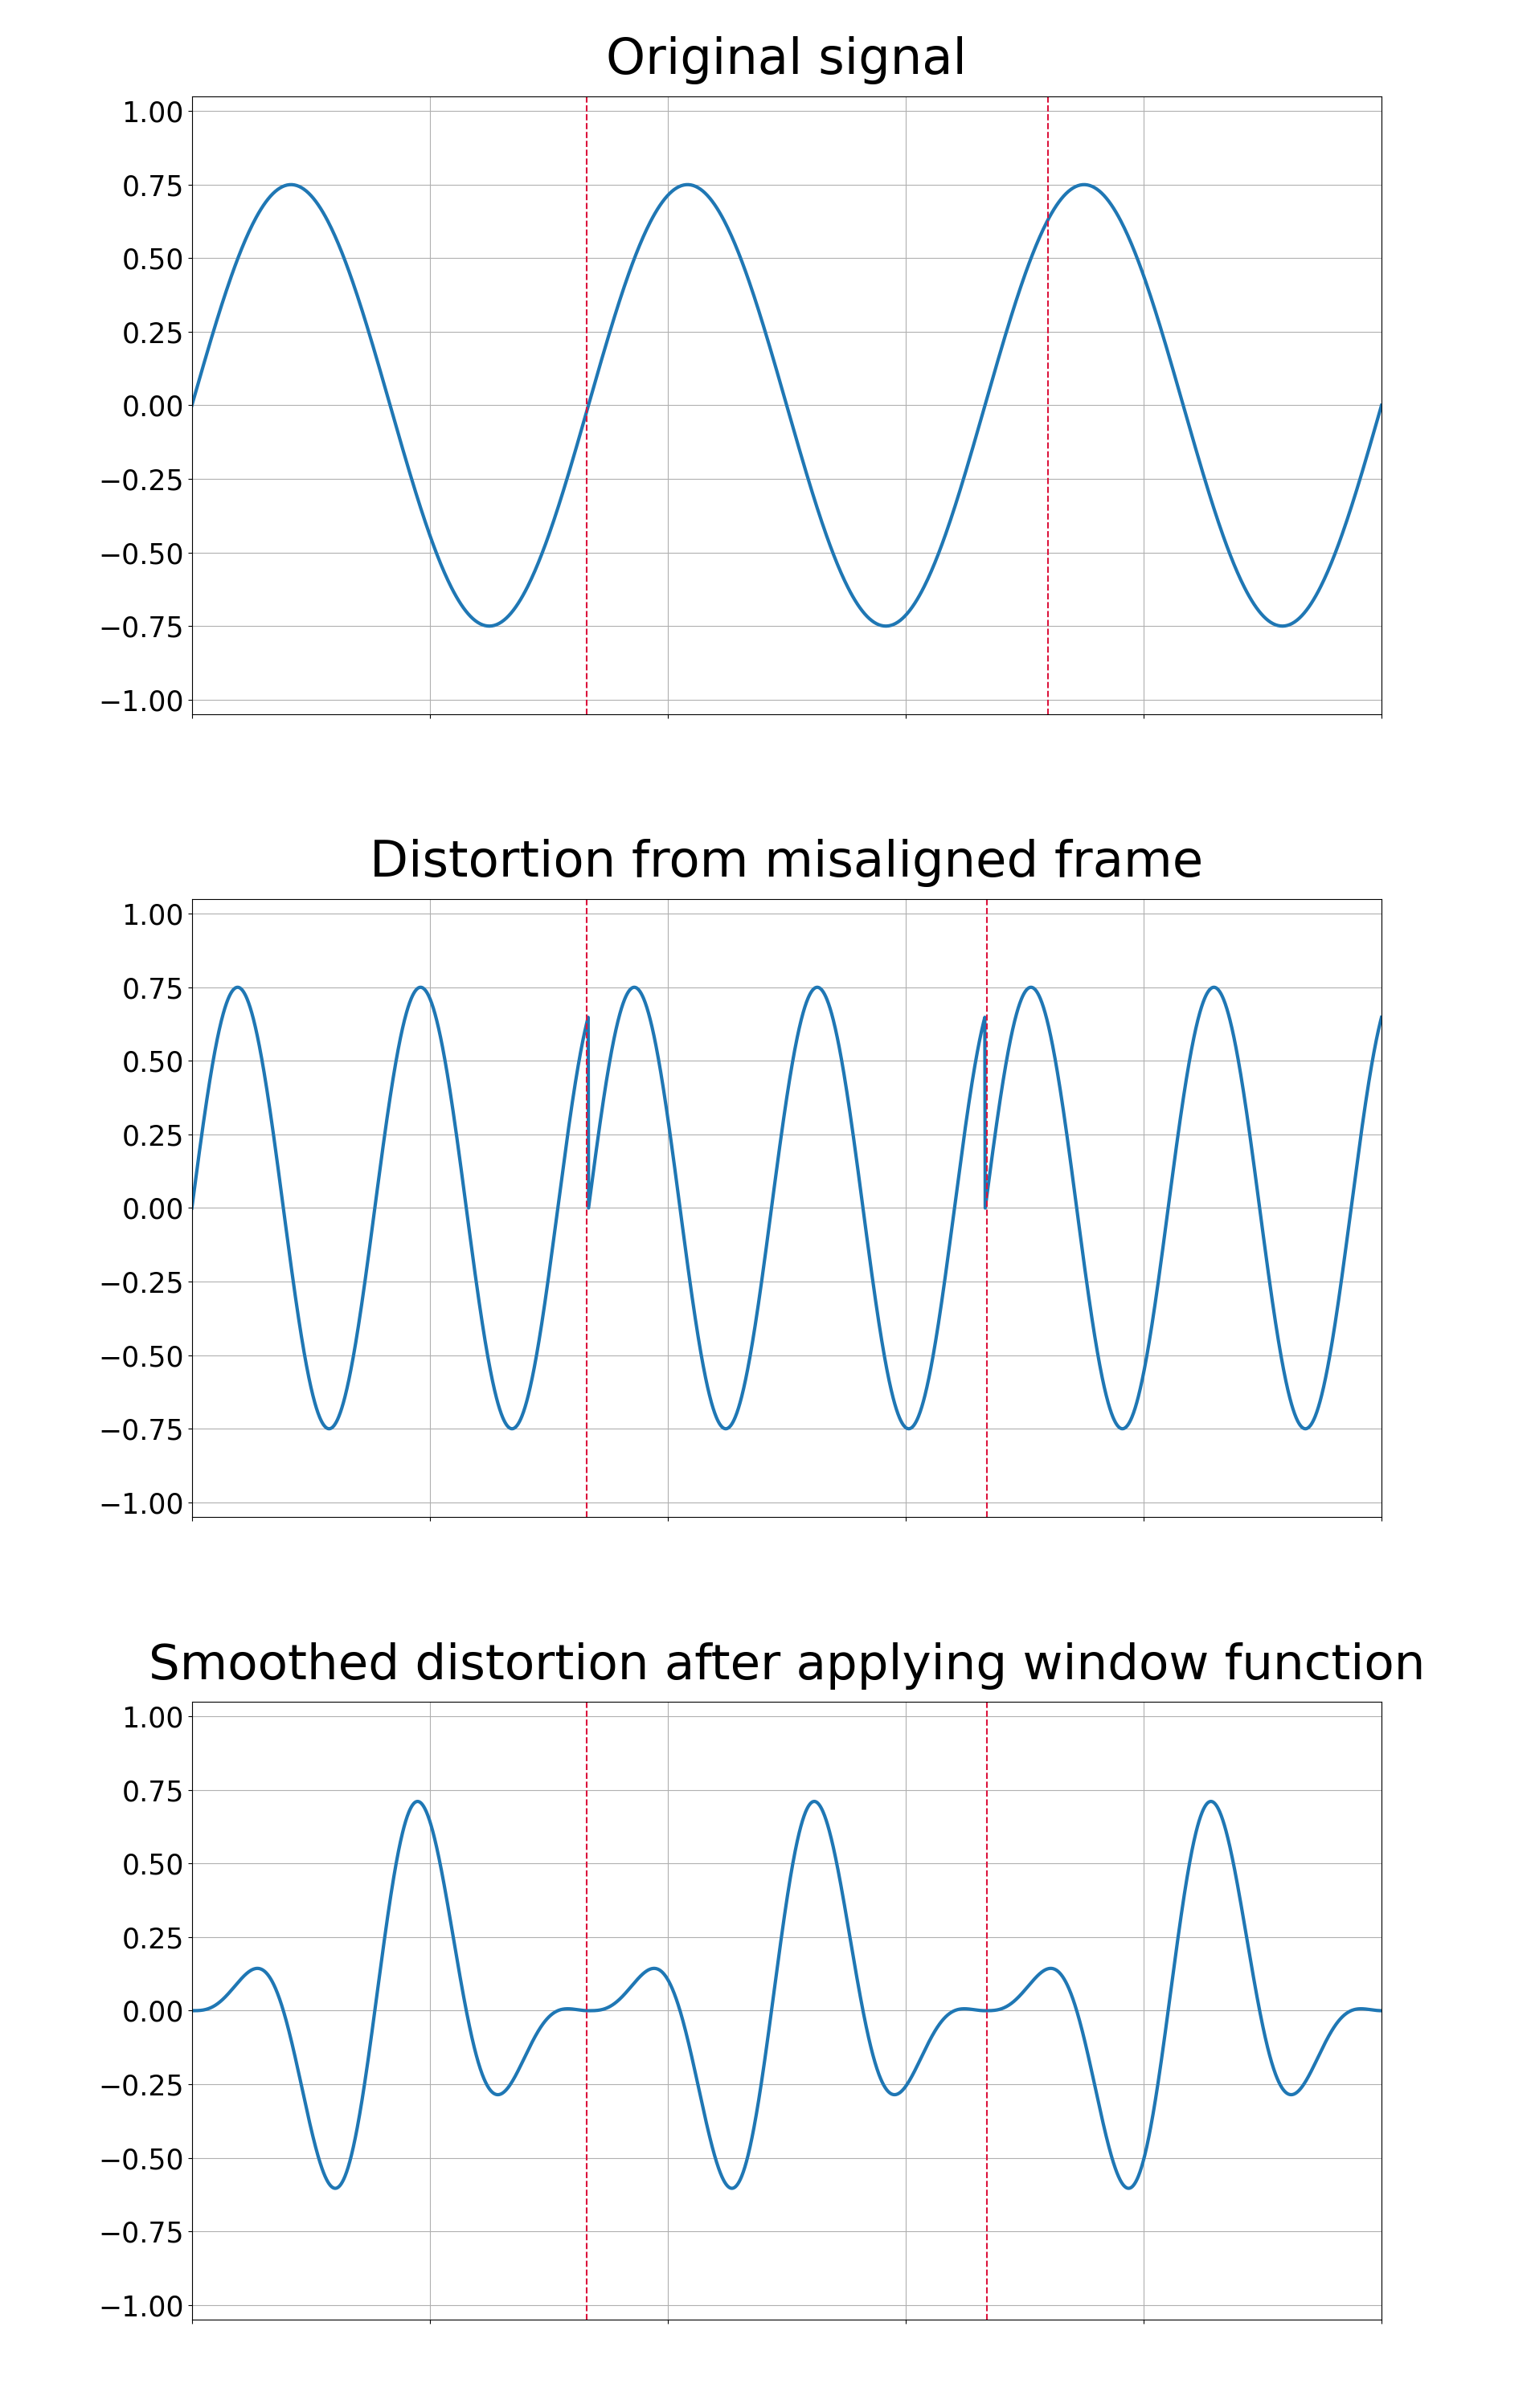
\includegraphics[width=\linewidth]{fig/framedistortion.png}
    \caption{Distortion caused by misaligned framing.}
    \label{fig:framedistortion}
\end{figure}

Given signal $s(n)$ and window function $w(n)$, we get the resulting windowed signal $\text{res}(n)$ using:
\[ \text{res}(n) = s(n) * w(n) \]
Figure~\ref{fig:windowfunc} shows the working of a window function on a frame graphically.
\begin{figure}[h]
    \centering
    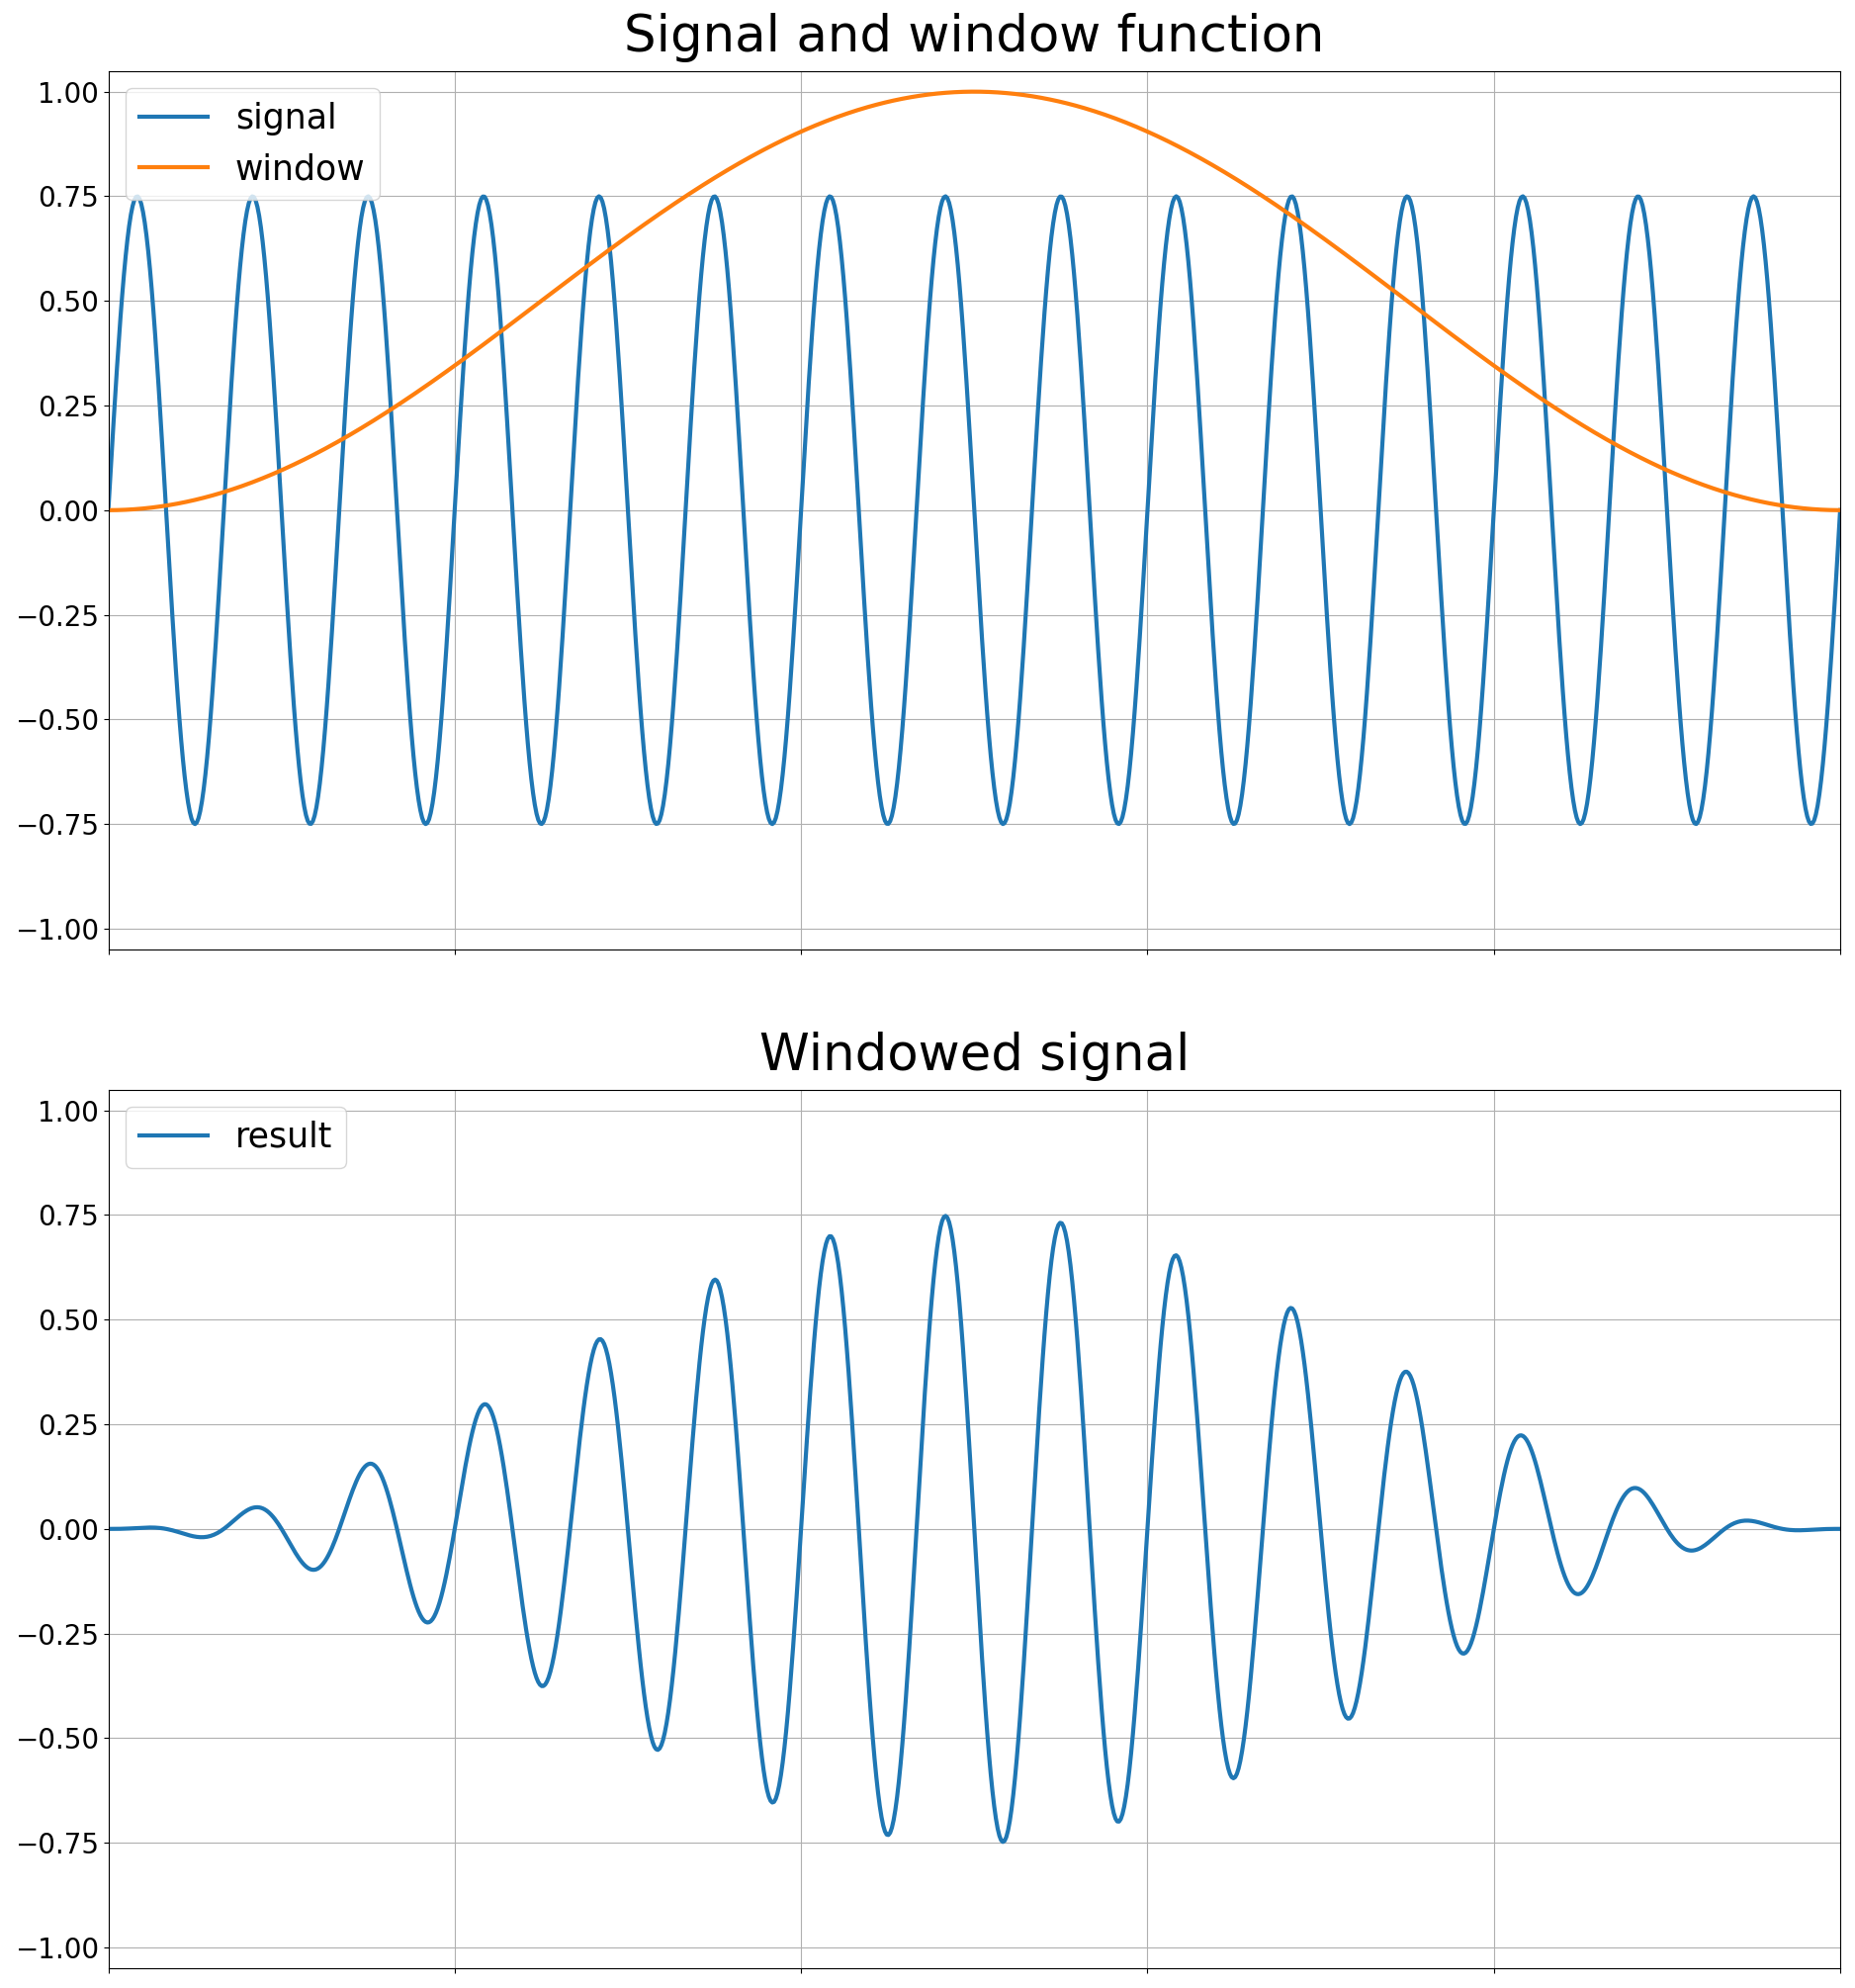
\includegraphics[width=\linewidth]{fig/window.png}
    \caption{An example of applying a window function to a signal.}
    \label{fig:windowfunc}
\end{figure}

The \textcolor{red}{characteristics} \textcolor{gray}{(TODO: better word)} of spectral leakage from framing can be controlled using different window functions.
%, see Figure~\ref{fig:windowfunceffect} for some examples.
Applying no window function is referred to as using a rectangular window, as all the "wanted" samples from the signal are multiplied by 1 and all other samples by 0, effectively framing the signal. We won't discuss individual window function in this section; see Appendix~\ref{sec:windows} for an in depth discussion on the different window functions.

The leakage behavior of a window function can be quantified by performing a Fourier transform on the window function. The resulting frequency domain shows the amount of leakage in neighboring bins compared to the power of the center bin. To show the leakage behavior of frequencies which do not align with a bin, we can zero-pad the window function, which causes over-sampling in the frequency domain. Zero-padding is further discussed in Section~\ref{sec:zeropadding}. Figure~\ref{fig:winleak} shows the leakage of a rectangular window when a frequency exactly matches the center frequency of a bin and the leakage when a frequency is exactly between bins. Here we can see the leakage spectrum has lobes of leakage. The lobe containing the center bin is called the main lobe and the other lobes are called side lobes. The different window functions trade-off between having a narrow main lobe width and low side lobe levels~\cite{windowfunc}.
\begin{figure*}[b]
    \centering
    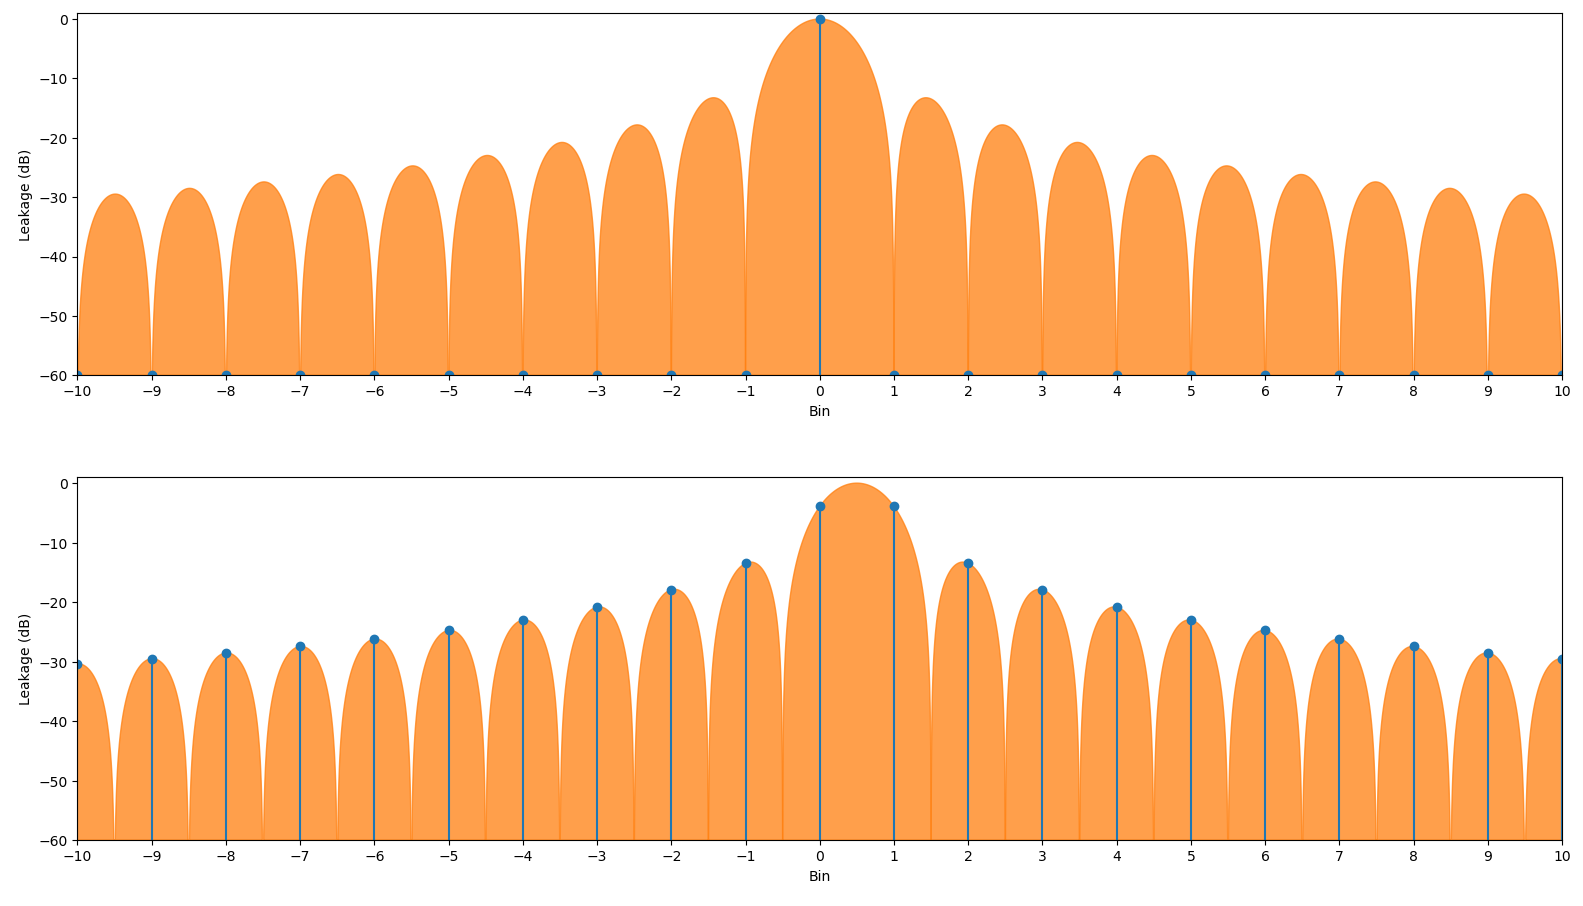
\includegraphics[width=\linewidth]{fig/winleak.png}
    \caption{\textcolor{red}{TODO: Better image.} Leakage behavior of the rectangular window. The orange lobes represent the frequency response of the rectangular window function; the blue lines represent the signal power measured in each bin given a signal frequency at the center of the main lobe of the frequency response of the window function. In the top plot, the frequency of the signal exactly matches the center frequency of a bin. If we then look at the leakage at every bin position, we see that all signal power goes into the center bin and nothing into any other bin. In the bottom plot, we shifted the frequency response half a bin up to simulate a frequency in the signal half a bin higher than some arbitrary bin. If we now look at the height of the frequency response at every bin position, we can see that the signal power diminishingly leaks into all subsequent bins.}
    \label{fig:winleak}
\end{figure*}

% Window functions alter the amplitude of the original signal. This causes...
The performance of window functions is often described using equivalent noise bandwidth, coherent power gain and scalloping loss~\cite{windowperf3, windowperf2, windowperf}. Equivalent noise bandwidth signifies the variation in noise floor compared to using a rectangular window. In other words, when transforming a signal, all the noise in the signal will result in some power in every bin, creating a floor in the spectrum. Window functions raise this noise floor by a consistent amount, which is quantified using equivalent noise bandwidth.
%
Applying a window function causes the overall amplitude of a frame to decrease, which in turn decreases the power of bins. This reduction is called the coherent power gain and signifies the loss of power in the spectrum.
%
As mentioned earlier, when a signal does not fit a frame, it leaks into other bins in the spectrum. Scalloping loss is the amount of decibel lost in the bin containing the main lobe when transforming a frame containing a signal halfway between bins compared to a signal right on a bin.
%
In order to accurately describe the signal power, we would need to correct for these effects. Equivalent noise bandwidth and coherent power gain can be described by a fixed value for each window function, but scalloping loss depends, along with the sample rate and frame size, on the spectral content of the signal, which we have no control over. On top of this, there are several other problems with accurate signal power estimation. Since absolute signal power estimations are not required for the content of this thesis, we will simply rely on relative power estimations.

\subsection{Real-time}
Real-time is a difficult concept, as it has multiple definitions based on what field of research it is used in. As the formal definitions relate to very different concepts, it usually does not cause any problems. Problems arise when the term is informally used, as the vernacular definitions often miss an important aspect of the formal definitions of real-time, which causes statements made about systems which adhere to these vernacular definitions to be unreliable or useless. Here are a few examples of different definitions (vernacular definitions are marked red):
\begin{enumerate}
    \item Being synced with actual clock time (or wall time). This is for instance relevant when playing media such as audio and video. When such media is played at an incorrect speed, it could be considered distorted. The hardware which keeps track of the clock time is called a real-time clock.
    \item A system must response within a specified time constraint, which is called the real-time constraint or deadline. This constraint is usually a relatively short time. This definition comes from real-time computing and is relevant when making car airbags or airplane control systems. Failing to response within the real-time constraint leads to failures of the system. Real-time systems are often classified into hard, firm and soft real-time based on the impact of missing the deadline~\cite{realclass}. 
    \color{red}\item\color{black} A system which can provide a result or feedback with no noticeable delay after receiving some input. Examples of such systems include graphical user interfaces or instant chatting/calling. There are no hard deadlines which the system has to respond within and the system does not fail if some delay does occur. Only user experience is slightly impacted. In the field of real-time computing, this is often referred to as near real-time.
    \color{red}\item\color{black} A system which can process data faster than it acquires data. This is technically not real-time, however, it is often used as such in academic literature. It is important for real-time systems to process data faster than it acquires data so it does not lag behind after some time, however, this is an implicit deadline. Not having this deadline explicit may lead to non-sensible expectations of the system.
\end{enumerate}
Even though the first definition is very relevant when working with audio, it is not relevant for us. The audio drivers of operating systems handle all timing for us. We simply have to wait for samples to be recorded and made available to our program. We only have to keep the sampling rate in mind when working with the samples as shown in the previous section.

% TODO: Maybe it's a firm real-time system. And usefulness degrades more if latency was higher.
In order to allow guitarists to use their guitar as a MIDI instrument, our system has to respond within a small time frame. On top of that, if the system fails to respond quickly enough, the usefulness of the result degrades, as timing is very important when playing an instrument. These restrictions would classify our system as a soft real-time system. We choose a real-time of constraint of \textcolor{red}{TODO} milliseconds. We elaborate on this choice in Section~\ref{sec:constraint}.

Other work in real-time pitch estimation often uses the forth definition of real-time. This is problematic when using Fourier transform based methods, as many papers choose large frame sizes to get a high resolution in the frequency domain. For instance, in order to discern the two lowest notes on a guitar which are 4.9 Hz apart, we would need a frame length of 204 milliseconds. This implicit deadline is well over our real-time constraint and would be unplayable for any musician. Other papers we found which do explicitly set a real-time constraint, choose very high constraints from 140 ms~\cite{sloomboi} up to 360 ms~\cite{sloomboi2}. These constraints were likely chosen with the inherent limits of their solutions in mind. It is very important to set a real-time constraint solely based on the expectation of the systems from an outside perspective. Real-time constraints chosen with the inner working of the system in mind are merely a measure of performance that is hoped to be achieved and claiming a system is real-time based on such constrains is considered fraudulent. We have found no papers Fourier transform based pitch estimation papers which choose a sensible real-time constraint.

\subsection{Music theory and notation}
In modern western music, we use the twelve-tone equal temperament (12-TET) music system. This system divides an octave, which is the interval between a pitch and another pitch with double the frequency, into twelve equally spaced semitones on the logarithmic scale. The logarithmic scale is used such that the perceived interval between two adjacent notes is constant~\cite{perception}. As a result, the ratio between two frequencies in an $n$-semitone interval is $\sqrt[12]{2}^n$ or $2^{\frac{n}{12}}$, invariant to pitch. A semitone can be further divided into 100 logarithmically scaled cents. %Cents are often used to measure the amount of dissonance.

Using scientific pitch notation, every note can be uniquely identified by combining the traditional note names \note{A}{} to \note{G}{} (with accidentals such as $\sharp$ and $\flat$) with an octave number (e.g. \noteflat{E}{3}). An octave starts at \note{C}{}, which means the octave number increases between \note{B}{} and \note{C}{}. This counter intuitively implies \note{A}{3} is higher than \note{C}{3}. Note that in 12-TET, \notesharp{C}{} and \noteflat{D}{} are enharmonically equivalent. In this thesis, we will always refer to the sharp ($\sharp$) note instead of the enharmonically equivalent flat note ($\flat$). %Furthermore, even though technically \notesharp{B}{3} (which is equal to \note{C}{4}) is within the fourth octave, it is denoted to be in the third octave as accidentals do not change the octave number.
The range of a typical electric guitar in standard tuning is from \note{E}{2} up to \note{E}{6}.

The 12-TET music system only describes the relation between two notes in an interval. In order to play with other musicians in harmony, an arbitrary note has to be tuned to a specific frequency. Per ISO 16, the standard tuning frequency of the \note{A}{4} is 440 Hz within an accuracy of 0.5 Hz~\cite{isoa}. In this thesis, we will always assume a 12-TET music system with a 440 Hz tuning note.

Using the above information, we can translate frequencies into scientific note names and vice versa. In order to numerically work with note names, we assign a value to each note as shown in Table~\ref{tab:notenames}.
\begin{table}[h]
    \hfill
    \begin{center}
        \begin{tabular}
        {l|l}
            name & number \\
            \hline
            \note{C}{}      & 0 \\
            \notesharp{C}{} & 1 \\
            \note{D}{}      & 2 \\
            \notesharp{D}{} & 3 \\
            \note{E}{}      & 4 \\
            \note{F}{}      & 5
        \end{tabular}
        \qquad
        \begin{tabular}{l|l}
            name & number \\
            \hline
            \notesharp{F}{} & 6 \\
            \note{G}{}      & 7 \\
            \notesharp{G}{} & 8 \\
            \note{A}{}      & 9 \\
            \notesharp{A}{} & 10 \\
            \note{B}{}      & 11
        \end{tabular}
    \end{center}
    \hfill
    \caption{The number corresponding to each note name}
    \label{tab:notenames}
\end{table}
In order to make calculations easier, we use \note{C}{0} as a tuning note instead of \note{A}{4}. We can calculate the frequency of \note{C}{0} using the fact that \note{C}{0} is 57 semitones lower than \note{A}{4}:
\begin{align*}
    f_{C_0} = f_{A_4} * 2^{\frac{-57}{12}} &= 440 * 2^{\frac{-57}{12}} \\
                                           &\approx 16.352 \text{ Hz}
\end{align*}
% \[ f_{C_0} = 440 * 2^{\frac{-57}{12}} = 16.352 \text{ Hz} \]
% \[ 440 * \sqrt[12]{2}^{-57} = 16.352 Hz \]

We can calculate the frequency $f_{N_O}$, where $N$ is the note name which is represented by a numerical value given by Table~\ref{tab:notenames} and $O$ is the octave number using:
\begin{align*}
    f_{N_O} &= f_{C_0} * 2^O * 2^{\frac{N}{12}} \\
            &= f_{C_0} * 2^{O + \frac{N}{12}}
\end{align*}
% \[ f_{N_O} = f_{C_0} * 2^O * 2^{\frac{N}{12}} \]

To calculate the closest note $N_O$ corresponding to a frequency $f$, we first calculate the number of semitones $n_s$ between the tuning note $f_{C_0}$ and $f$:
\begin{align*}
    n_s = \round{12 * {}^{2}\!\log{\frac{f}{f_{C_0}}}}
\end{align*}
% Or more generally given a tuning note $N_O$:
% \begin{align*}
%     n_s^{N_O}(f) = \round{12 * {}^{2}\!\log{\frac{f}{f_{N_O}}}}
% \end{align*}
Here, $\round{\ldots}$ denotes rounding to the nearest integer. By rounding, we find the closest note to $f$. Now we can calculate $N$ and $O$ as follows:
\begin{align*}
    N &= n_s \mod 12 \\
    O &= \floor{\frac{n_s}{12}}
    % O &= n_s / 12
\end{align*}
Note that we assume $a \mod b$ always return a number $c$ for which $0 \leq c < b$. Some programming languages allow the modulo operator to return a value $c$ for which $-b < c < b$, resulting in $-13 \mod 10 = -3$ instead of $-13 \mod 10 = 7$. Furthermore, when using a conversion to an integer instead of a floor, the octave number is rounded up when the note distance is negative.

In order to calculate the error $e$ (in cents) between the given frequency to the closest tuned note, we first calculate the tuned frequency $f_t$ of the closest note:
\[ f_t = f_{C_0} * 2^{\frac{n_s}{12}} \]
Then the error $e$ can be calculated using:
\[ e = 1200 * {}^{2}\!\log{\frac{f}{f_t}} \]

In digital music processing, notes are often represented through MIDI note numbers. A MIDI note number can take a value from 0 to 127. The MIDI standard defines \note{C}{4} to be MIDI note number 60. This makes the standard tuning frequency \note{A}{4} number 69 and \note{C}{0} number 12.

The MIDI note number $m$ corresponding to the note closest to frequency $f$ can be calculated using the semitone distance from a frequency with a known MIDI note number. Let $m(N_O)$ denote the MIDI note number of $N_O$:
\begin{align*}
    m &= \round{12 * {}^{2}\!\log{\frac{f}{f_{N_O}}}} + m(N_O)% \\
      % &\approx \round{12 * {}^{2}\!\log{\frac{f}{16.352}}} + 12 \\
      % &= \round{12 * {}^{2}\!\log{\frac{f}{f_{C_0}}}} + 12
\end{align*}
Conversely, the frequency $f$ of the note corresponding to MIDI number $m$ can be calculated as follows:
\begin{align*}
    f &= f_{N_O} * 2^{(m - m(N_O)) / 12}% \\
      % &\approx 16.352 * 2^{(m - 12) / 12} \\
      % &= f_{C_0} * 2^{(m - 12) / 12}
\end{align*}

% \subsection{Science of sound}  \label{sec:physsound}
\subsection{Physical properties of sound}  \label{sec:physsound}
The perceived loudness of a note over time can be described using an ADSR envelope. The ADSR envelope of a played note is the convex hull of the waveform of the signal, see Figure~\ref{fig:adsr} for an example. This convex hull can be divided into four parts: Attack, Decay, Sustain and Release. When a note is strummed on the guitar, a percussive sound is generated which causes a loud and sharp attack along with the note. This percussive sound quickly decays and only the actually fretted note will sustain. Finally, when the note is released, it dies out quickly.
\begin{figure}[h]
    \centering
    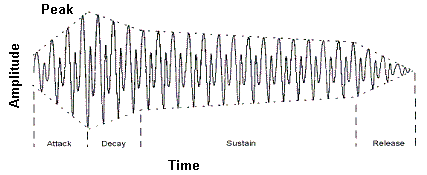
\includegraphics[width=\linewidth]{fig/envelope.png}
    \caption{Example of an ADSR envelope \textcolor{red}{(TODO: Better image)}.}
    \label{fig:adsr}
\end{figure}

The percussive sound generated when strumming a note is called a transient. Transients contain a high degree of non-periodic components. Because of this, transients appear very chaotically in the frequency domain and are often considered noise. As a transient is of high amplitude, it overshadows the note which will eventually sustain. Consequently, we cannot use the samples from a transient for Fourier based pitch estimation. This in turn increases our minimum latency, as we have to wait for samples which do not contain the transient anymore.

When playing a note on an instrument, many sine waves are generated. The most notable frequency is called the fundamental frequency and determines what note is actually played. Integer multiples of the fundamental frequency can resonate and give rise to harmonic overtones~\cite{overtones}. In practice, these overtones are not exact integer multiples due to non-linear effects.

Many other frequencies are generated along with the fundamental and its overtones. The instrument specific pattern of these frequencies, along with the characteristics of the overtones, is called the timbre of the instrument~\cite{timbre}. The timbre is what differentiates the sound of the same note played on two different instruments~\cite{perception}. Generally, the amplitude of the timbre frequencies is low compared to the fundamental frequency and can be disregarded as noise in the frequency domain. Figure~\ref{fig:timbre} shows the effect of timbre on a waveform.
\begin{figure}[h]
    \centering
    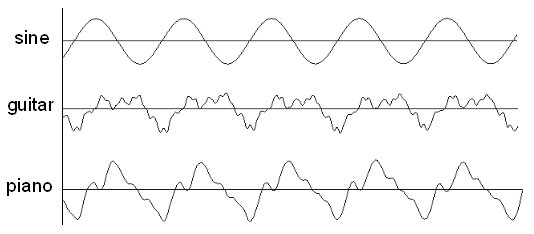
\includegraphics[width=\linewidth]{fig/timbre.jpg}
    \caption{Example of difference in timbre between instruments compared to a sine wave.}
    \label{fig:timbre}
\end{figure}

In Section~\ref{sec:related}, we mentioned overtones are dissonant with respect to notes in 12-TET. This is true for all overtones, except for octaves, which are all overtones numbers equal to $2^n - 1$ for every $n$. In Table~\ref{tab:overseries}, we show an example for the overtones of \note{C}{4}. Note that the series of errors is always the same, regardless of what the starting note is. 
\begin{table}[h]
    \centering
    \begin{tabular}{rrcrr}
        $n$ & $f_{\text{overtone}}$ & closest note & $f_\text{note}$ & error \\
        \hline
        0 & 261.626  & $C_4$    & 261.626  &  - \\
        1 & 523.251  & $C_5$    & 523.251  &  0 \\
        2 & 784.877  & $G_5$    & 783.991  &  1.955 \\
        3 & 1046.502 & $C_6$    & 1046.502 &  0 \\
        4 & 1308.128 & $E_6$    & 1318.510 &  -13.686 \\
        5 & 1569.753 & $G_6$    & 1567.982 &  1.955 \\
        6 & 1831.379 & $A^\#_6$ & 1864.655 &  -31.174
    \end{tabular}
    \caption{Example of overtone series from \note{C}{4} and the errors compared to the closest note}
    \label{tab:overseries}
\end{table}

\textcolor{red}{TODO: Rewrite.}
As mentioned in Section~\ref{sec:related}, when using the CQT transform, none of the non-octave overtones coincides with a CQT bin as the CQT bins are exponentially spaced like the notes in a scale. This causes the frequencies of the overtones to spread out over bins, resulting in more noise in the frequency domain. Furthermore, overtones are important for discerning fundamentals from noise generated by transients. By using a Fourier transform tuned to a specific note, all its overtones are also coincide with Fourier bins. By performing a Fourier tuned to every note in the 12 tone scale, we can measure every note and its overtones.

\textcolor{gray}{TODO: This thesis mainly focuses on monophonic pitch estimation, as it is much easier to perform. But we can still see how well our strategy works in the polyphonic case.
TODO: A big problem in monophonic pitch estimation is the octave problem. Octaves are difficult to discern as the fundamental frequency and overtones of the higher note coincide with the overtones of the lower note. A similar problem arises
TODO: The main problem in polyphonic pitch estimation comes from the occurrence of overtones. As mentioned before, notes in octave tend overshadow each other. Furthermore, as shown in Table~\ref{tab:overtones}, the overtones of a note can coincide with the...
TODO: Overtone overlap and polyphonic difficulty.}
\begin{table}[h]
    \centering
    \hfill
    \begin{tabular}{r|l}
        $n$ & $f^{C_3}_0*n$ \\
        \hline
        1 & 130.813 \\
        2 & 261.626 \\
        \textcolor{red}{3} & \textcolor{red}{392.438} \\
        4 & 523.251 \\
        \textcolor{blue}{5} & \textcolor{blue}{654.064}
    \end{tabular}
    \hfill
    \begin{tabular}{r|l}
        $n$ & $f^{E_3}_0*n$ \\
        \hline
        1 & 164.814 \\
        2 & 329.628 \\
        3 & 494.441 \\
        \textcolor{blue}{4} & \textcolor{blue}{659.255} \\
        5 & 824.069
    \end{tabular}
    \hfill
    \begin{tabular}{r|l}
        $n$ & $f^{G_3}_0*n$ \\
        \hline
        1 & 195.998 \\
        \textcolor{red}{2} & \textcolor{red}{391.995} \\
        3 & 587.993 \\
        4 & 783.991 \\
        5 & 979.989
    \end{tabular}
    \hfill
    \caption{Overtones of C, E and G}
    \label{tab:overtones}
\end{table}
\begin{table}[h]
    \centering
    \begin{tabular}{c|c|c}
        Note & $f$ & $\Delta f$ \\
        \hline
        $f^{C_3}_2$ & 392.438 & \multirow{2}{*}{0.443} \\
        $f^{G_3}_1$ & 391.995 & \\
        \hline
        $f^{C_3}_4$ & 654.064 & \multirow{2}{*}{5.191} \\
        $f^{E_3}_3$ & 659.255 &
    \end{tabular}
    \caption{Colliding overtones}
    \label{tab:diff}
\end{table}


\section{Real-time Fourier transform based monophonic pitch estimation}
At the heart of our research lies a pitch estimation algorithm. The task of a pitch estimation algorithm is to convert a frame of samples to some representation of the notes contained in the frame. In this thesis, we will focus on spectral analysis methods of pitch estimation. Specifically, we focus on pitch estimation using the spectra obtained from frames using the Fourier transform.

% We will start with constructing a very basic pitch estimation algorithm. Then we will 

% \textcolor{gray}{When working in real-time, actions which are normally trivial have to be analyzed critically. For instance, sleep when retrieving samples from audio in, non-blocking overlap number of samples to carry over...}

% \textcolor{gray}{Actual research etc. Summary what was done in the research project which we build on. Notes on future work of research project.}

% \textcolor{gray}{As mentioned in Section~\ref{sec:related} and shown in our research project, the resolution in the frequency domain is not sufficient for spectral peak selecting methods. Given the info in preliminaries, we can tune Fouriers to specific frequencies.}

\subsection{Real-time constraint}  \label{sec:constraint}
Before we start constructing our pitch estimation system, let us first choose a real-time constraint. The goal of our pitch estimation system is creating a digital representation of the played notes so it can for example be used for software sound synthesis. Consequently, the real-time constraint should reflect the critical latency. This is the latency for which delay between playing a note and receiving the feedback, such as hearing back the synthesized note, becomes problematic. The critical latency is highly subjective and may even differ between playing styles.
% Therefore, we will deduce a reasonable real-time constraint from multiple upper bounds stemming from different arguments.
% Therefore, we will deduce a reasonable real-time constraint from a few different arguments.
Note that our real-time constraint only considers pitch estimation latency. If we want to do anything with the pitch estimation results in real-time, such as synthesizing audio, additional latency will be introduced. For this reason, we shouldn't put our real-time constraint right at the critical latency, but leave some headroom for the program using our estimated pitches.

Even though the critical latency is subjective, it is the factor determining if a real-time pitch estimation system is usable in musical context. In order to determine the critical latency empirically, we created a tool called \textit{delayed playback}, which plays back recorded audio with an arbitrary latency. Using \textit{delayed playback}, we found a latency of \textcolor{red}{TODO} milliseconds is a reasonable latency at which we can still comfortably play many songs. \textit{Delayed playback} can also be used to verify if a real-time constraint chosen by someone else is reasonable by your own standards. The tool is described in depth in Section~\ref{sub:playback_latency}.% Note that the reported latency from does not include the latencies introduced by the audio drivers and hardware discussed in Section~\ref{sub:computer_audio}.

% \textcolor{gray}{TODO: Rewrite paragraph, as playing faster is easier due to relying more on muscle memory instead of listening to yourself.}
The critical latency depends, among other things, on the speed with which notes are played. For instance, let's assume a latency of 50 milliseconds. When playing a slow song consisting of quarter notes at 120 BPM, resulting in 2 notes per second, the latency is only a tenth of the note duration. However, when playing a fast solo consisting of sixteenth notes at 210 BPM, resulting in 12 notes per second, the latency is 70\% of the note duration. This means you hear more of the previous note than the current note for the duration with which the current note is played, which makes playing at fast speeds extra difficult. % This tricks the brain in such a way that it prevents you from staying on beat.

There is a limit on how fast we can estimate the pitch of a played note. For instance, when we consider transients noise, we have to wait for the transient to pass before we can gather samples containing the note. Then, we need enough samples such that the lowest bin of the DFT doesn't exceed the frequency of the lowest note. In the case of \note{E}{2}, which is 82.407 Hz, we would need a minimum frame length of $ \frac{1}{82.407} * 1000 = 12.135 $ milliseconds. Due to spectral leakage, using such small frame lengths is not feasible. However, as outlined in Section~\ref{sub:waveform_packet}, we can translate this idea to the time domain. In practice, this would result in a minimum latency of 14 to 15 milliseconds.

In order to assess what we can reasonably expect from our system, we measured the latency of a commercial guitar synthesizer solution. This is described in depth in Appendix~\ref{sec:ax100}. Here, we found the Axon AX 100 MKII at worst has a latency of 15 milliseconds when it is able to guess the note "the first try". Otherwise, the latency may reach up to 40 milliseconds.

\textcolor{gray}{TODO: Note on unaccounted latencies (audio driver/hardware latencies).}
A careful reader may have noticed we actually discussed two different latencies. We mostly reason about the latency of our pitch estimation system. However, when reasoning about the critical latency, latencies from the audio driver and hardware as discussed in Section~\ref{sub:computer_audio} do matter. \textcolor{gray}{TODO: Estimate on these latencies. Estimate of latency when running Digistring's algorithms on specialized hardware}.

\textcolor{gray}{TODO: Our real-time constraint choice.}

% \textcolor{gray}{Start with the factors coming into play when choosing the real-time constraint for our system (latency, played notes per second etc). Note on measured latency in Appendix~\ref{sec:ax100}. Empirically found bounds on latency using our latency program}

% \subsection{Software amplification}
% \textcolor{gray}{(Software representation of samples and FFT). The FFT works on floating point numbers but most audio interfaces give up to 24 bit integers...}
% \textcolor{gray}{We found empirically that when amplifying the input signal in software, peaks in the frequency domain are much easier to detect. However, it has to be done carefully to prevent distortion artifacts.}

\subsection{Basic algorithm for pitch estimation}
Let us start with constructing the most basic Fourier based monophonic pitch estimation algorithm. Here, we simply return the note closest to the bin with the highest magnitude. Every frame, we try to read a full frame of samples from the audio driver and apply a window function to the frame. To minimize our latency, we want to choose our frame size as small as possible while still being able to discern the two closest notes in frequency a typical guitar can produce. Due to the exponential nature of notes, the lowest two notes are always the closest two. For a typical guitar, these notes are \note{E}{2} and \note{F}{2}, which have a corresponding frequency of 82.407 Hz and 87.307 Hz respectively. This means we need a frequency resolution of at least $87.307 - 82.407 = 4.9$ Hz. This equates to a frame length of $4.9^{-1} = 0.204$ seconds, or 204 milliseconds. The bin centers do not have to exactly align with the notes to be able to discern them, so in practice we could get away with slightly shorter frames. Still, such large frame lengths are problematic for multiple reasons. A frame will contain multiple played notes when a guitarist plays at a moderate tempo (playing eighth notes in 150 BPM corresponds to 200 millisecond notes). Furthermore, if a frame contains the start of note, the whole frame might be useless due to the transient. Lastly, since we have to wait until the audio driver has enough samples ready for us to fill a frame, the first samples from that frame will be 200 milliseconds old. The average latency of processing a sample is 100 milliseconds due to the frame length alone. This is well over our real-time constraint.

We implemented this basic Fourier pitch estimation algorithm in Digistring (\texttt{BasicFourier Estimator}). The corresponding pseudo code is given in Algorithm~\ref{alg:basic_pitch}. On average, the pitch estimation is performed in 0.4 milliseconds. This means our limiting factor is the long frame lengths, which implies we should look for methods which allow for accurate pitch estimation with lower frequency resolution. Furthermore, especially on low pitched notes, it often picks the note one octave higher than the fundamental frequency. Apart from the octave errors, the pitch estimator often does produce correct results, however, it is completely infeasible for real-time usage due to the low frame rate. As we only produce one note estimate for every frame, we essentially quantize our estimator to eight notes on 150 BPM.
\input{pseudo_code/basic_pitch.pc}

\subsection{Overlapping frames}
As seen in the previous section, a low frame rate is problematic, as our note output rate is synced to the frame processing rate, essentially quantizing our note estimation to the frame processing rate. The straightforward solution would be to decrease the frame length. However, the frame length is limited by the minimum frequency resolution we need. Instead, we can increase the frame rate by partially overlapping subsequent frames.

Overlapping has several advantages. Apart from the increased frame rate, which decreases accidental quantization, it may decrease the average latency of processing a sample. Furthermore, as transients are very short in the time domain, having more frames over a certain period of time decreases the relative number of frames containing the transient, which causes more frames to have a useful note estimate, see Figure~\ref{fig:overlap_transient} for a graphical explanation.
\begin{figure}[h]
    \centering
    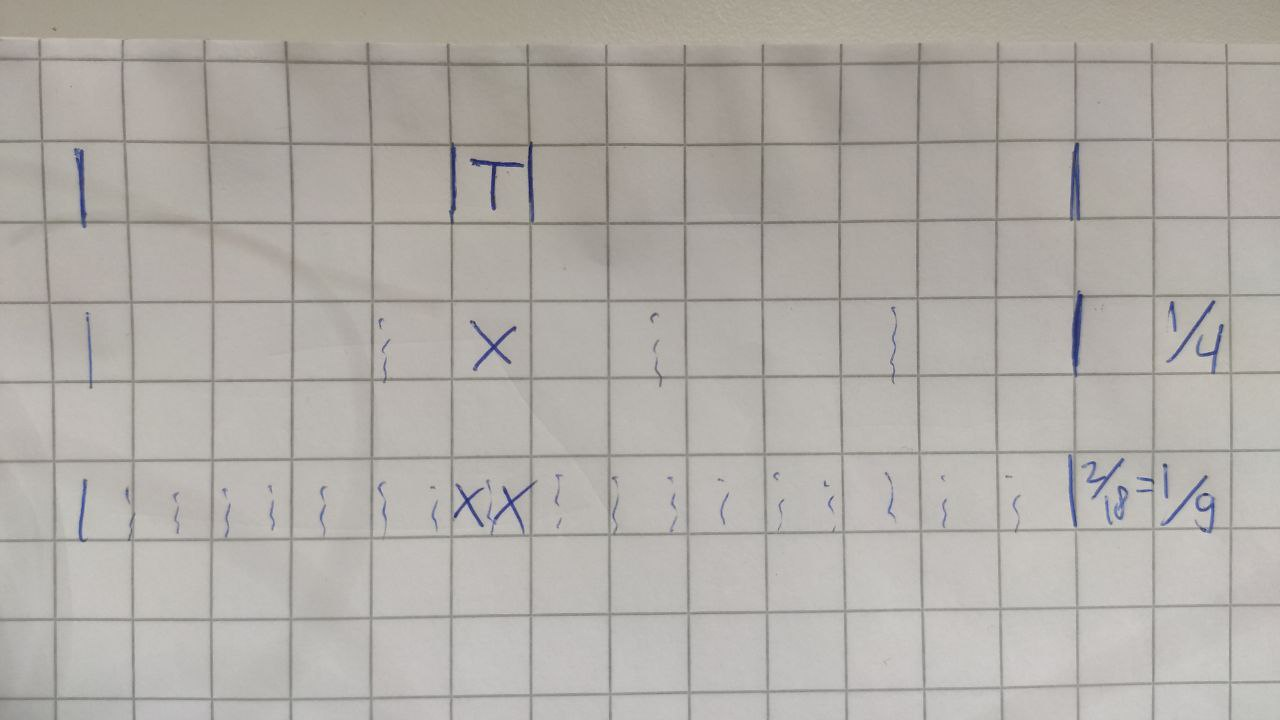
\includegraphics[width=\linewidth]{fig/overlap_transient.jpg}
    \caption{\textcolor{red}{TODO: Correct image showing overlap instead of just shorter frames.} Given the signal given on top with a transient at T, relatively less frame estimations are ruined by the transient when using a higher frame rate.}
    \label{fig:overlap_transient}
\end{figure}

As two subsequent frames share information when overlapping, the estimation from subsequent frames is correlated. This limits the usefulness of overlapping beyond a certain overlap ratio~\cite{overlap}. However, as long as we don't overlap so much that samples are gathered faster than we can process them, overlapping doesn't incur an addition latency on the pitch estimation system.

When performing real-time estimation, instead of overlapping a constant ratio between frames, we can overlap based on the rate at which the audio driver acquires samples and our previous frame processing time. Time spend waiting for samples is effectively wasted time, as that time could've been spent on generating note estimations. Instead, we can always retrieve all currently available samples from the audio driver and fill the rest of the frame with samples from the previous frame. This ensures maximum possible overlap every frame.

\subsection{Zero padding}  \label{sec:zeropadding}
The number of output bins is determined by the number of samples that is transformed. We can artificially increase the number of samples in a transform by appending zeros to the frame. This technique is called zero padding. As only silence is added to the frame, it does not alter the spectrum.

As mentioned in Section~\ref{sec:fourier}, the frequency resolution of a DFT is $\Delta f_{bin} = \frac{f_{\text{SR}}}{n_F}$. Let $n_{F_P}$ be the zero padded frame size. Given that the sample rate is constant, our frequency resolution will increase by a factor of $\frac{n_{F_P}}{n_F}$. In other words, if we zero pad the frame such that it becomes $x$ times larger, our frequency resolution will increase by a factor $x$.

It is important to note that zero padding does not increase the resolution of the DFT, as no extra information about the original signal is added to the frame. It merely interpolates the coarse spectrum to become more smooth~\cite{zeropad1}. Two frequencies closer than $\Delta f_{bin}$ together form one big lobe in the smoothed spectrum~\cite{zeropad2}. However, the interpolated peaks may have a higher amplitude than the original peaks, thus improving the results of our basic pitch estimation algorithm. See Figure~\ref{fig:visualpadding} for a graphical example of this.

Zero padding is relatively compute intensive form of interpolation~\cite{interpolnozero}.% The time complexity of the DFT is $O(N^2)$, where $N$ is the frame size. In the case of the FFT, the time complexity is reduced to $O(N \log N)$.
\begin{figure}[h]
    \centering
    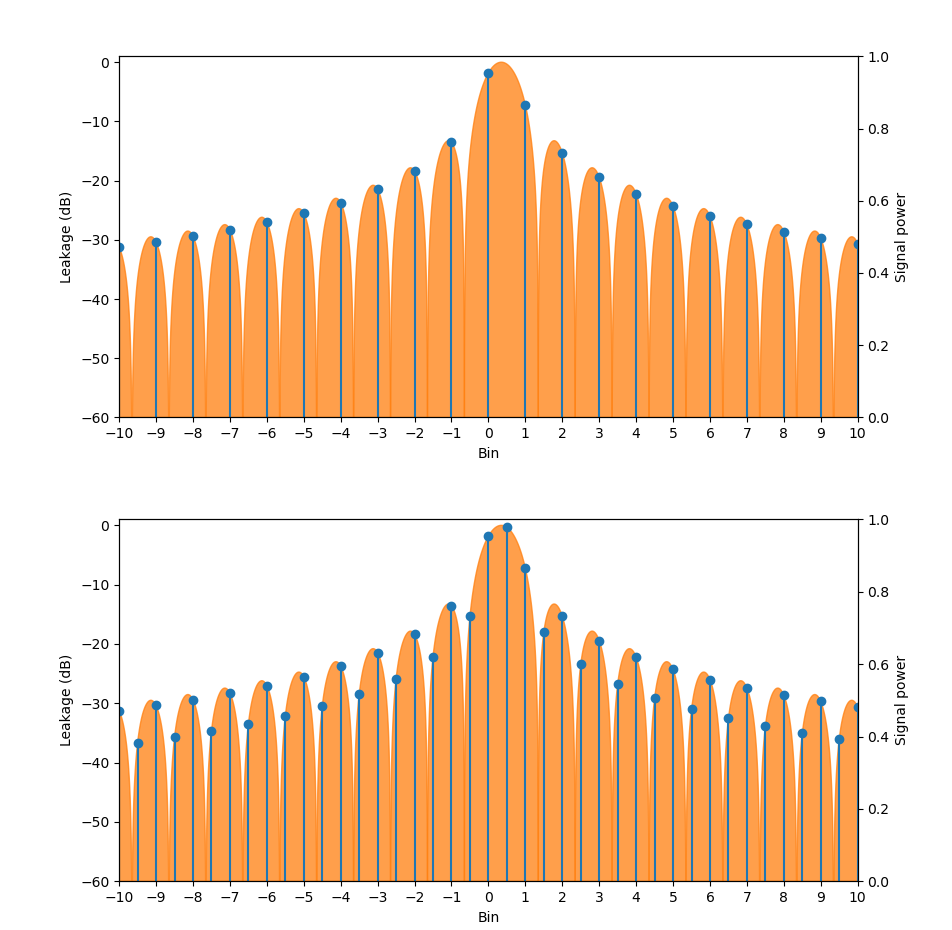
\includegraphics[width=\linewidth]{fig/zero_pad_interpolate.png}
    \caption{\textcolor{red}{TODO: Better image.} Left and right figure show DFT spectrum without and with zero padding respectively. The blue lines represent the bin magnitudes. Here, $n_{F_P} = 2 * n_F$. The orange lobes represent the frequency content of the frame if infinite zero padding was applied.}
    \label{fig:visualpadding}
\end{figure}

\subsection{Quadratic interpolation}
A less compute intensive method of interpolation is quadratic interpolation, also know as Quadratically Interpolated FFT (QIFFT)~\cite{interpolnozero}. Given a peak bin and its neighbors, QIFFT interpolates the actual peak location by fitting a parabola through these three points. The vertex of the fitted parabola is the interpolated peak location.

The accuracy of interpolation can be improved by performing the interpolation on a logarithmically-weighted magnitude spectrum (LQIFFT). In other words, the error of interpolation is reduced if the logarithm of the bin power is used. Since a Gaussian curve is a parabola on a logarithmic scale, the interpolation is nearly perfect when using a Gaussian window function on a unweighted spectrum~\cite{interpolgaus}. It isn't perfect, as a true Gaussian window would need infinite long tails~\cite{gauswin}.

\textcolor{gray}{XQIFFT?}

To perform the interpolation, we calculate a value $p \in [-\frac{1}{2}, \frac{1}{2}]$, which is the offset in bins of the interpolated peak with respect to the peak bin $b_j$. Using the magnitude of the peak $|b_j|$ and the magnitude of the neighboring bins $|b_{j - 1}|$ and $|b_{j + 1}|$, we define:
\begin{align*}
    \alpha &= w(|b_{j - 1}|) \\
    \beta  &= w(|b_{j}|) \\
    \gamma &= w(|b_{j + 1}|)
\end{align*}
Here, $w(x)$ is an arbitrary weighting function. In the case of LQIFFT:
\[ w(x) = \ln{x} \]
Then, we can calculate $p$ as follows:
\[ p = \frac{1}{2} \cdot \frac{\alpha - \gamma}{\alpha - 2\beta + \gamma} \]
The weighted amplitude $a_i^w$ corresponding to the interpolated peak is:
\[ a_i^w = \beta - \frac{(\alpha - \gamma) * p}{4} \]
The non-weighted interpolated amplitude is:
\[ a_i = w^{-1}(a_i^w) \]
Here, $w^{-1}(x)$ is the inverse of $w(x)$. In the case of LQIFFT:
\[ w^{-1}(x) = e^{x} \]
Given the bin number $j$ of the spectral peak location, the frequency $f_i$ corresponding to the interpolated peak is:
\[ f_i = \Delta f_{bin} * (j + p) \]

Quadratic interpolation can be combined with zero-padding for better results~\cite{interpolnozero}.

\subsection{Peak picking}

Gaussian peak picking. Min-max peak picking. Peak filtering.

\subsection{Note selection from peaks}
Different strategies to select notes from peaks.

\subsection{High resolution estimator}
Most basic Fourier based estimator. Base algorithm (apply Fourier, calc norms, pick peaks, find notes in peaks, ...).\\
Different peak pickers, note finders (in peaks) and note set filtering

\subsection{Tuned Fourier transforms}
12 Fouriers for each note and it's overtones.


\section{Digistring}
\textcolor{gray}{Details about the program I've written. Usage instructions, code choices, code structure, screenshots, expandability}
TODO!!! Our framework provides scientist willing to research real-time pitch estimation an efficient implementation of many basic functions (e.g. efficient overlapping buffers, debug wave form generation, note synthesis based on estimation).

\textcolor{gray}{General Digistring structure}

\textcolor{gray}{Subsections with details of implementations. E.g. sample getting (sample format conversion in real time, sleeping, etc.), (Overlap frames for more context. Small caveat; if Estimator is unaware of overlapping, it may find notes completely in the past which weren't found when those samples were the present), no accurate amplitude measurement but make everything relative to loudest measured signal, audio synthesis (no plopping techniques), Estimators+EstimatorGraphics}
Lastly, experimentation is difficult... Many ways to report note estimations and all datasets have different annotation standard (solved using intermediate representation). Automatically calculates commonly used performance measures. Ambiguity of performance measure (all are both good and bad).

\subsection{Playback latency}  \label{sub:playback_latency}
\textcolor{gray}{Details on how we made the playback latency tool.}


\section{Experiments}  \label{sec:exp}
\textcolor{gray}{Note that the parameters were empirically optimized with informal experiments. Datasets. Actual experiments.}


\section{Conclusions}
\textcolor{gray}{What we did in this thesis. Reflection on the performance of the system. Final reference to the source code.}


\section{Future work}  \label{sec:future}
\textcolor{gray}{What could still be improved/further researched.}

\subsection{Waveform packets}  \label{sub:waveform_packet}
Low frequency tones from a guitar come in "packets". By detecting the distance between two packets, we can estimate the frequency.



\appendix
\section{Measuring the latency of the AXON AX 100 mkII}  \label{sec:ax100}
\textcolor{gray}{Lekker meten en weten.}

\section{Effect of different window functions}  \label{sec:windows}
\textcolor{gray}{Plots met effect van verschillende window functions. Rectangular narrowest main lobe and least ENBW. The Hann window is an all round performing window and as a result is often used. The Welch window is a window with a very narrow center lobe. The Dolph–Chebyshev window has little and very evenly spread overall leakage (optimal filter). Parzen window (and b-spline windows per extension) have much space between lobes (lobe density. }
% for ENBW of different windows: https://www.gaussianwaves.com/2020/09/equivalent-noise-bandwidth-enbw-of-window-functions/

\begin{figure}[h]
    \centering
    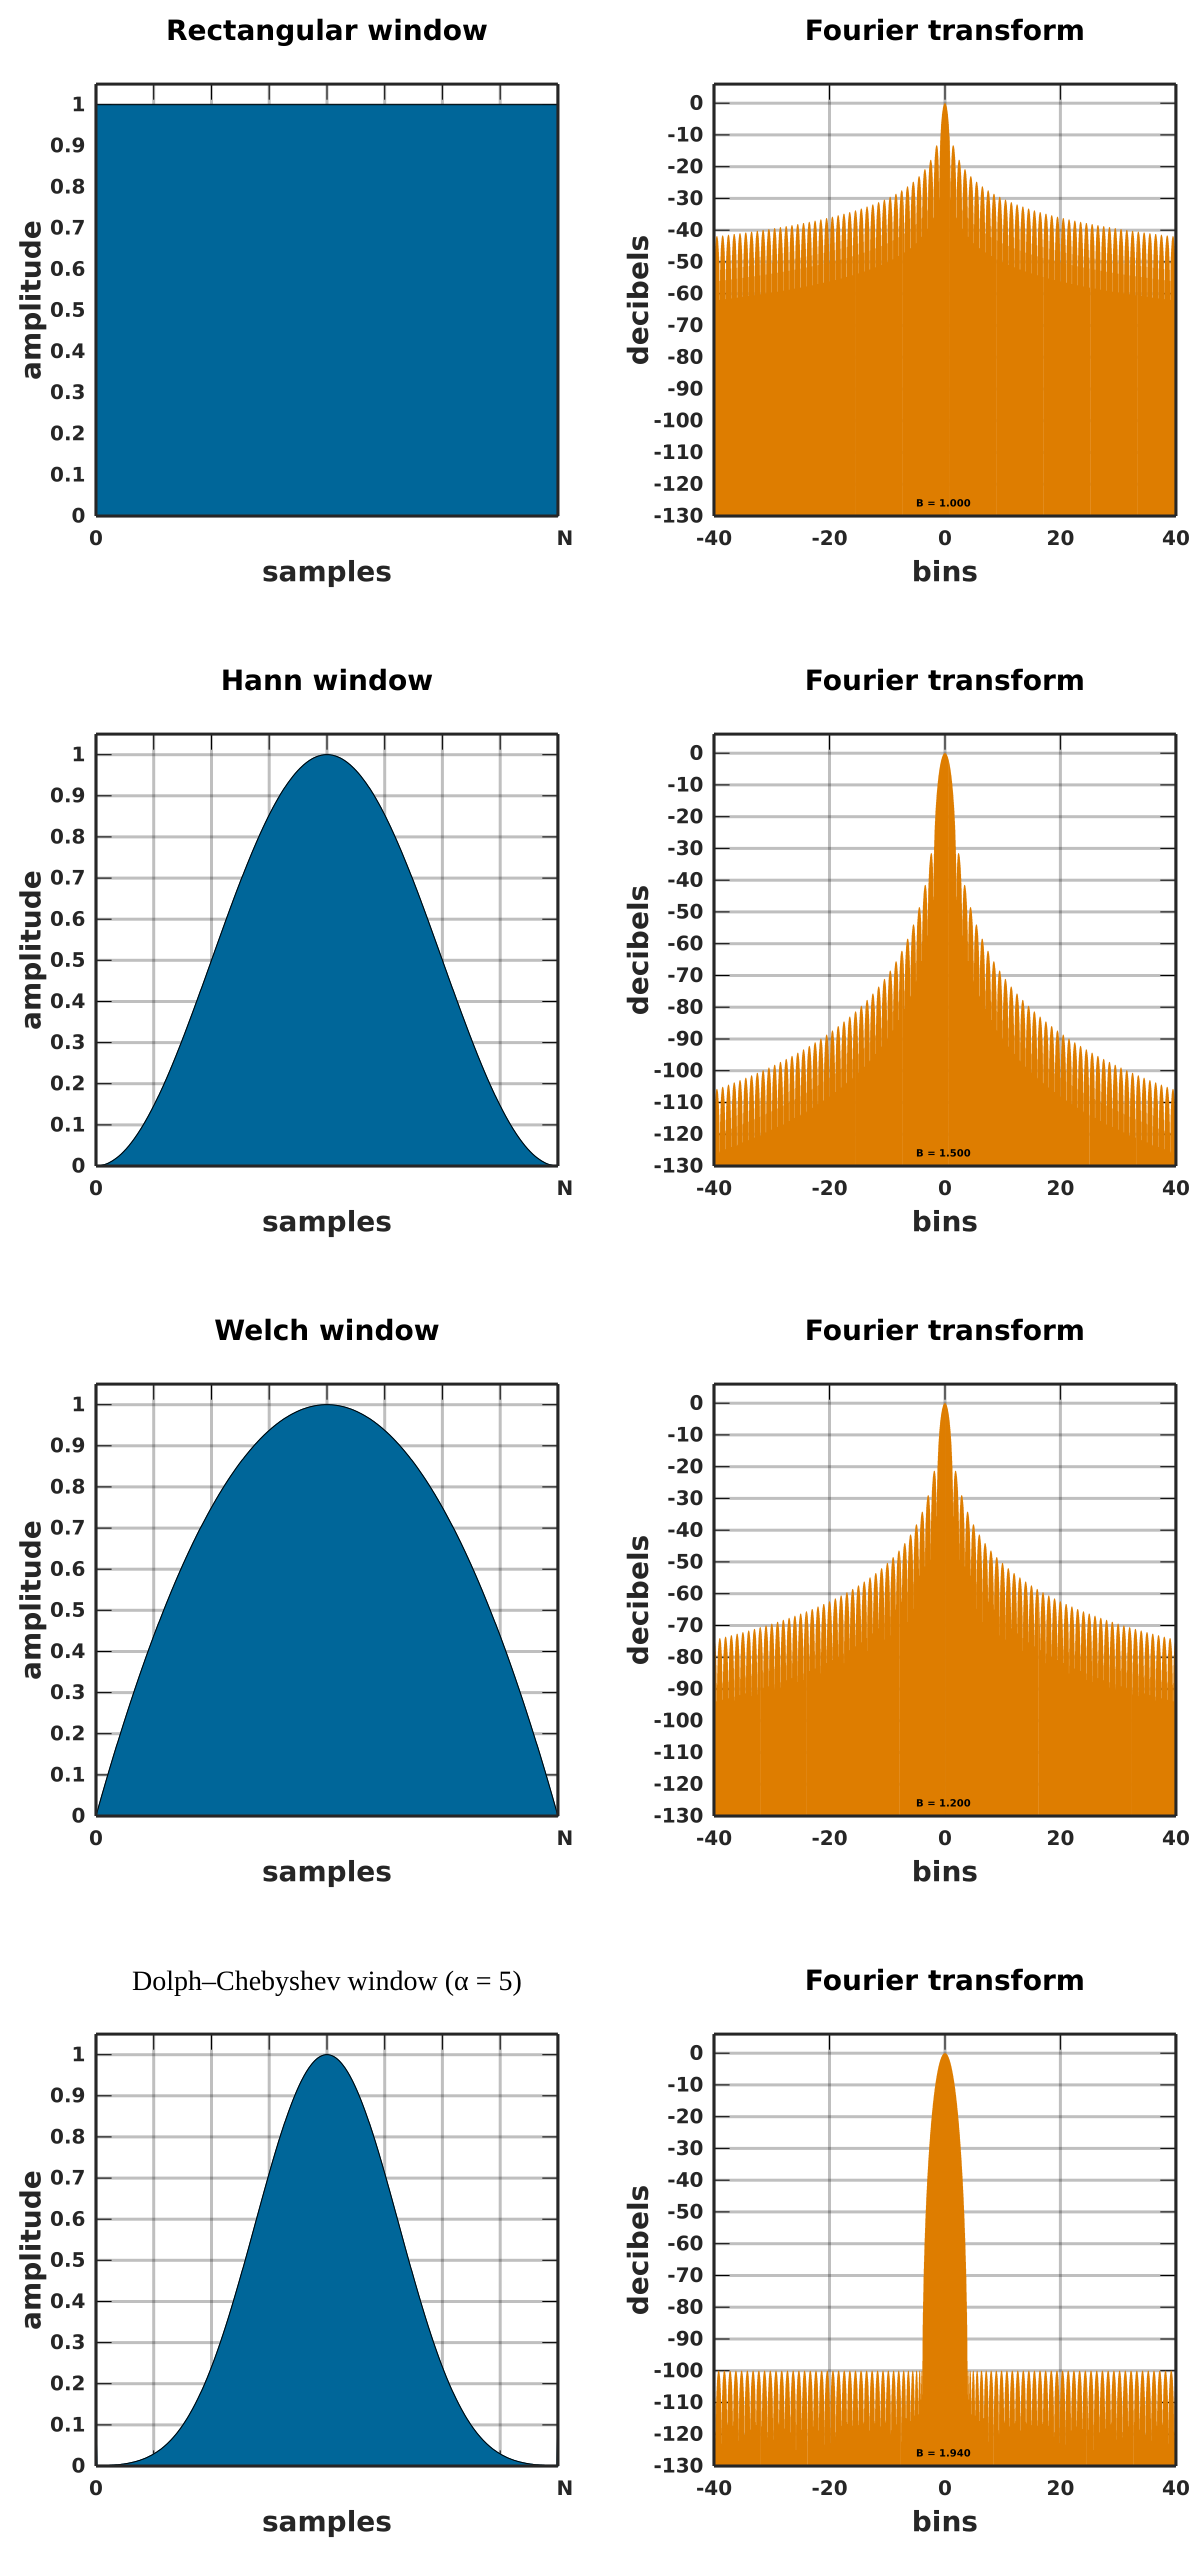
\includegraphics[width=\linewidth]{fig/windows.png}
    % 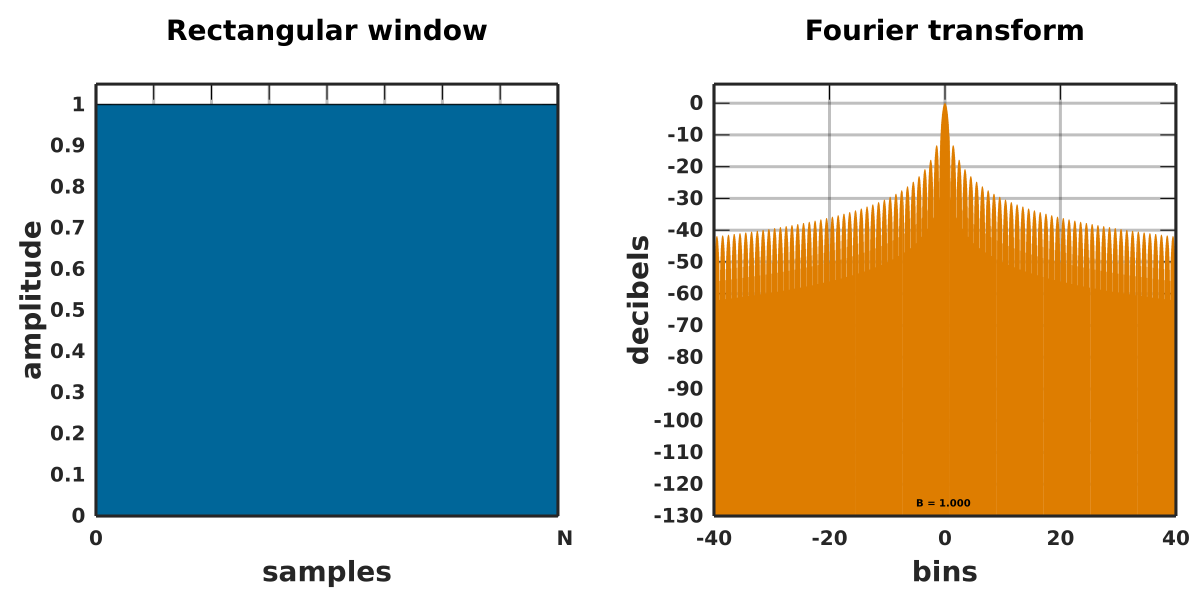
\includegraphics[width=\linewidth]{fig/window_rect.png}
    % 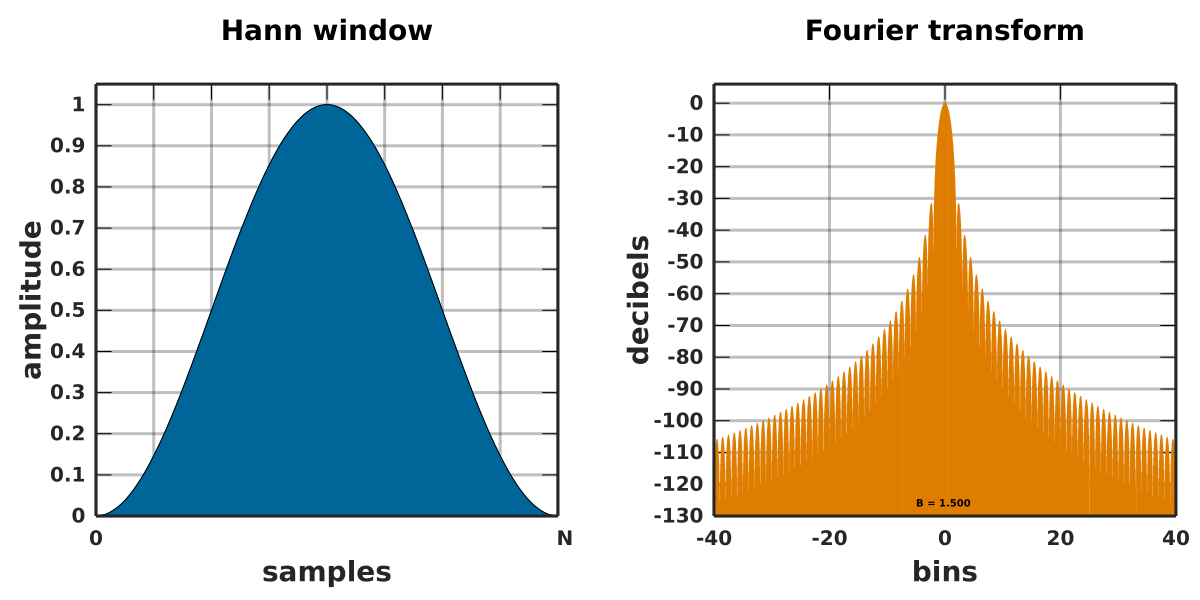
\includegraphics[width=\linewidth]{fig/window_hann.png}
    % 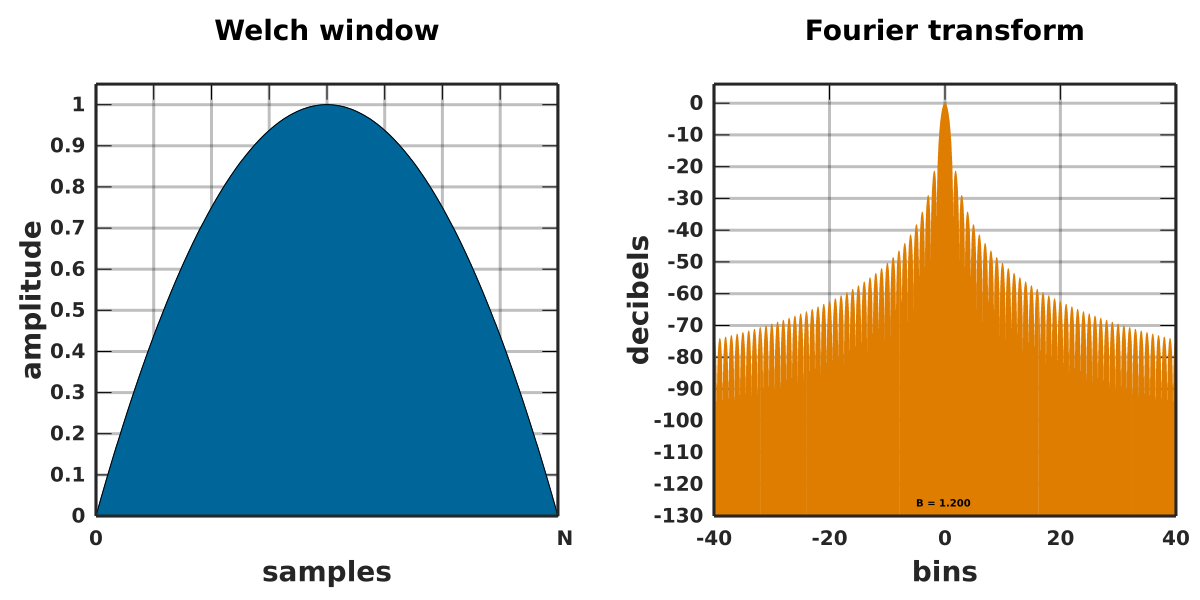
\includegraphics[width=\linewidth]{fig/window_welch.png}
    % 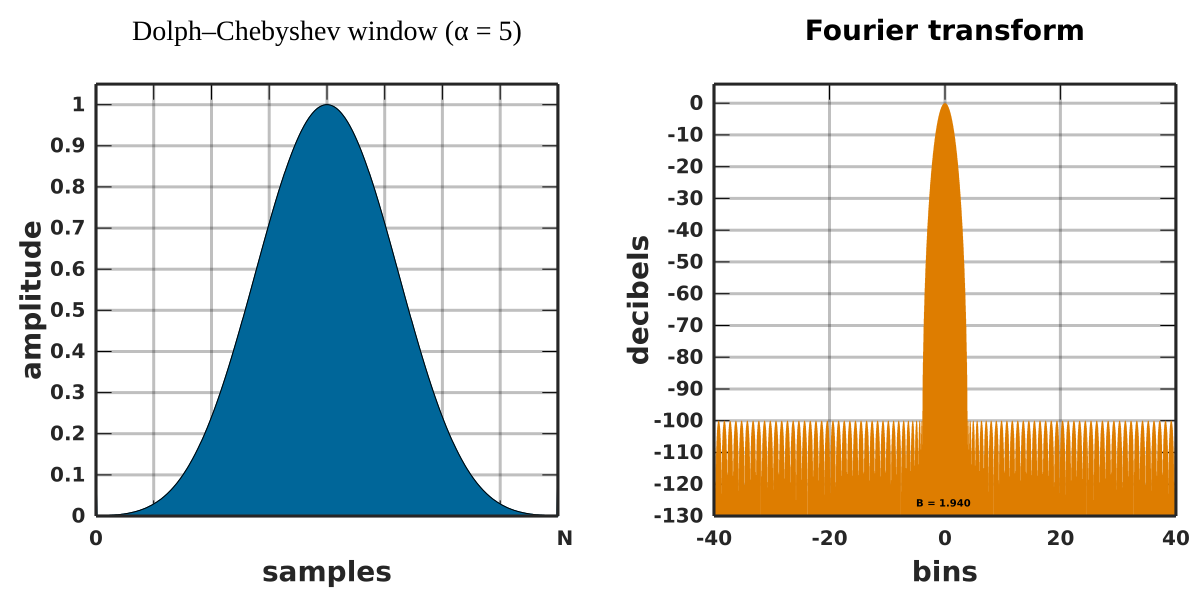
\includegraphics[width=\linewidth]{fig/window_dolph.png}
    \caption{Examples of the spectral leakage of some window functions.}
    \label{fig:windowfunceffect}
\end{figure}



\addcontentsline{toc}{section}{Bibliography}
\bibliographystyle{plain}
% \bibliographystyle{alpha}
\bibliography{thesis}

\end{document}
 